\documentclass[12pt]{acmart}

\usepackage[english]{babel}
\usepackage{amsmath, amsfonts, amsthm}
\usepackage{graphicx}
\usepackage{float}


\begin{document}

\begin{titlepage}
\title{lab2.3}
\author{Kosakian, Inozemtsev}
\date{}
\maketitle % Заголовок
\thispagestyle{empty}
\end{titlepage}

\tableofcontents
\newpage




\section{Ensemble methods}
    Multiple machine learning algorithms can be used to obtain better predictive performance than any of the constituent learning algorithms alone. A number of different ensemble methods have been proposed, such as Boosting, Bagging and Stacking.
    Boosting refers to a family of algorithms that are able to transform weak learners to strong learners. Bagging means training the same classifier on different subsets of same dataset. Stacking combines various classification via a meta-classifier (Aburomman \& Reaz, 2016). The base level models are built based on a whole training set, then the meta-model is trained on the outputs of the base level model as attributes.
    Jabbar et al. proposed an ensemble classifier which is built using Random Forest and also the Average One-Dependence Estimator (AODE which solves the attribute dependency problem in Naïve Bayes classifier. Random Forest (RF) enhances precision and reduces false alarms (Jabbar et al., 2017). Combining both approaches in an ensemble results in improved accuracy over either technique applied independently.
    \subsection{Hybrid based techniques}
        Traditional IDSs have limitations: that they cannot be easily modified, inability to identify new malicious attacks, low accuracy and high false alarms. Where AIDS has a limitation such as high false positive rate. Hybrid IDS is based on the combination of SIDS and AIDS. A Hybrid IDS overcomes the disadvantage of SIDS and AIDS. Farid et al. (Farid et al., 2010) proposed hybrid IDS by using Naive Bayes and decision tree based and achieved detection rate of 99.63\% on the KDD’99 dataset Figure \ref{fig1} .
        \begin{figure}[H]
            \centering{
            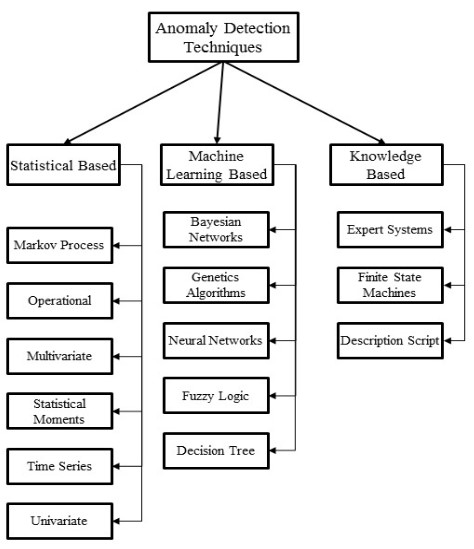
\includegraphics[width=130mm]{Picture1.png}
            }
            \caption{Taxonomy of Anomaly-Based Intrusion Detection}
            \label{fig1}
        \end{figure}
    \subsection{Performance metrics for IDS}
        There are many classification metrics for IDS, some of which are known by multiple names. Table \ref{tab1} shows the confusion matrix for a two-class classifier which can be used for evaluating the performance of an IDS. Each column of the matrix represents the instances in a predicted class, while each row represents the instances in an actual class. IDS are typically evaluated based on the following standard performance measures:\\
        \begin{center}
            Table 1 – Confusion Matrix for IDS System
            \label{tab1}
            \begin{tabular}{|c|c|c|c|}
                \hline
                &Predicted Class &  &\\
                \hline
                Actual Class & Class&Normal&Attack\\
                \hline
                & Normal & True Negative (TN) & False Positive (FP)\\
                \hline
                &Attack&False Negative (FN)&True Positive (TP)\\
                \hline
            \end{tabular}
        \end{center}
        \begin{itemize}
            \item Src\_bytes: Number of data bytes transferred from source to destination in a single connection.
            \item Dst\_bytes: Number of data bytes transferred from destination to source in a single connection.
            \item Flag: Status of the connection, i.e., Normal or Error.
            \item Count: Number of connections to the same destination host as the current connection in the past two seconds.
            \item Srv\_count: Number of connections to the same service (port number) as the current connection in the past two seconds.
            \item Same\_srv\_rate: The percentage of connections that were to the same service, among the connections aggregated in Count.
            \item Dst\_host\_count: Number of host connections to the destination
            \item Dst\_host\_srv\_count: Number of services connecting to the destination.
        \end{itemize}
        \begin{enumerate}
            \item True Positive Rate (TPR): It is calculated as the ratio between the number of correctly predicted attacks and the total number of attacks. If all intrusions are detected then the TPR is \ref{f1} which is extremely rare for an IDS. TPR is also called a Detection Rate (DR) or the Sensitivity . The TPR can be expressed mathematically as:\\
            $$f(x)=a_0+\sum_{n=1}^\infty\Biggl(a_n\cos{\frac{n\pi}{L}}+b_n\sin{\frac{n\pi}{L}}\Biggr)\eqno(1)\label{f1}$$
            \item   False Positive Rate (FPR): It is calculated as the ratio between the number \ref{f2} of normal instances incorrectly classified as an attack and the total number of normal instances.
            $$y(x)=\sum_{i=1}^r\phi_i(x)y^i\eqno(2)\label{f2}$$
            \item False Negative Rate (FNR): False negative means when a detector fails to identify an anomaly and classifies it as normal \ref{f3}. The FNR can be expressed mathematically as:
            $$\phi_i(x)=\frac{\prod_{j=1}^d\mu_A{_j^i}(x_i)}{\sum_{k=1}^r\prod_{j=1}^d\mu_A{_{j(x_i)}^i}}\eqno(3)\label{f3}$$
            \item Classification rate (CR) or Accuracy: The CR measures how accurate the IDS is in detecting normal or anomalous traffic behavior \ref{f4}. It is described as the percentage of all those correctly predicted instances to all instances:
            $$Accuracy=\frac{TP+TN}{FP+FN+TP+TN}\eqno(4)\label{f4}$$
            where TP,TN – True Positive, True Negative;\\
            FP, FN – False Positive, False Negative.\\
            Receiver Operating Characteristic (ROC) curve: ROC has FPR on the x-axis and TPR on the y-axis. In ROC curve the TPR is plotted as a function of the FPR for different cut-off points. Each point on the ROC curve represents a FPR and TPR pair corresponding to a certain decision threshold. As the threshold for classification is varied, a different point on the ROC is selected with different False Alarm Rate (FAR) and different TPR. A test with perfect discrimination (no overlap in the two distributions) has a ROC curve that passes through the upper left corner (100\% sensitivity, 100\% specificity). The ROC Curve is shown in Figure \ref{fig2}.
            \begin{figure}[H]
                \centering{
                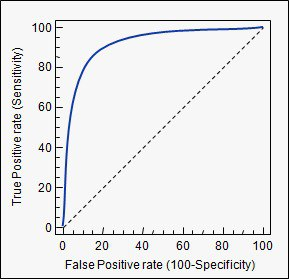
\includegraphics[width=130mm]{Picture2.png}
                }
                \caption{ROC curve}
                \label{fig2}
            \end{figure}   
        \end{enumerate}
    \subsection{Intrusion detection datasets}
        The evaluation datasets play a vital role in the validation of any IDS approach, by allowing us to assess the proposed method’s capability in detecting intrusive behavior. The datasets used for network packet analysis in commercial products are not easily available due to privacy issues. However, there are a few publicly available datasets such as DARPA, KDD, NSL-KDD and ADFA-LD and they are widely used as benchmarks. Existing datasets that are used for building and comparative evaluation of IDS are discussed in this section along with their features and limitations.
\end{document}
